\documentclass[11pt,a4paper]{report}

% Aberstwyth dissertation LaTeX Template
% Authors: Dr. Hannah Dee (hmd1@aber.ac.uk), Neil Taylor (nst@aber.ac.uk)
% This has been adapted from the Leeds Thesis template and the 
% Group Project template for Computer Science in Aberystywth University.
% 
% All comments and suggestions welcome.
%
% Template designed to be used with pdflatex: it may need alteration to
% run with a different LaTeX engine

% To build document on the unix command line, run four commands:
 
% pdflatex dissertation
% bibtex dissertation
% pdflatex dissertation
% pdflatex dissertation

% you will end up with dissertation.pdf 
\usepackage{mmp}
\usepackage{longtable}
\usepackage[normalem]{ulem}
\usepackage{caption}
\usepackage{float}
\usepackage{listings}
\usepackage{pdfpages}



\lstset{
    breaklines=true
}



% the following packages are used for citations - You only need to include one. 
%
% Use the cite package if you are using the numeric style (e.g. IEEEannot). 
% Use the natbib package if you are using the author-date style (e.g. authordate2annot). 
% Only use one of these and comment out the other one. 
\usepackage{cite}
%\usepackage{natbib}

% Use the following to selectively exclude chapters
%\includeonly{cover,abstract,acknowledge,declare,chapter1,chapter2}

\begin{document}

% all of the include directives below refer to tex files
% so 
\title{FIXME - the name of your project}

% Your name
\author{FIXME}

% Your email 
\authoremail{FIXME@aber.ac.uk}

\degreeschemecode{G400} %e.g. G400 
\degreeschemetitle{Computer Science} % e.g. Computer Science
\degreetype{BSc}

\modulecode{CS39440} % i.e. CS39440, CC39440, CS39620
\moduletitle{Major Project} % i.e. Major Project or Minor Project

\date{6th March 2012} % i.e. the date of this version of the report

\status{Draft} % Use draft until you create the release version. Then, change this to Release.
\version{1.0}

%The title and name of your supervisor.
\supervisor{Dr./Prof. My Supervisor} 

%The email for your supervisor. 
\supervisoremail{FIXME@aber.ac.uk}

\maketitle



 includes cover.tex - to change the content,
% edit the tex file

\pagenumbering{roman}

% This is the front page

\title{FIXME - the name of your project}

% Your name
\author{FIXME}

% Your email 
\authoremail{FIXME@aber.ac.uk}

\degreeschemecode{G400} %e.g. G400 
\degreeschemetitle{Computer Science} % e.g. Computer Science
\degreetype{BSc}

\modulecode{CS39440} % i.e. CS39440, CC39440, CS39620
\moduletitle{Major Project} % i.e. Major Project or Minor Project

\date{6th March 2012} % i.e. the date of this version of the report

\status{Draft} % Use draft until you create the release version. Then, change this to Release.
\version{1.0}

%The title and name of your supervisor.
\supervisor{Dr./Prof. My Supervisor} 

%The email for your supervisor. 
\supervisoremail{FIXME@aber.ac.uk}

\maketitle



                        

% Set up page numbering
\pagestyle{empty}

% declarations of originality 
\thispagestyle{empty}

%%%
%%% You must sign the declaration of originality. 
%%%
\begin{center}
    {\LARGE\bf Declaration of originality}
\end{center}

In signing below, I confirm that:

\begin{itemize}
\item{This submission is my own work, except where clearly
indicated.  }

\item{I understand that there are severe penalties for plagiarism 
and other unfair practice, which can lead to loss of marks
or even the withholding of a degree. }
 
\item{I have read the sections on unfair practice in the Students' 
Examinations Handbook and the relevant sections of the 
current Student Handbook of the Department of Computer 
Science.}
 
\item{I understand and agree to abide by the University's
regulations governing these issues.}
\end{itemize}

\vspace{3em}
Signature ............................................................  \\

\vspace{1em}
Date ............................................................ \\

%%% 
%%% We would like to make a selection of final reports available to students that take 
%%% this module in future years. To enable us to do this, we require your consent. You 
%%% are not required that you do this, but if you do give your consent, then we will have 
%%% the option to select yours as one of a number of reports as examples for other 
%%% students. If you would like to give your consent, then please include the following 
%%% text and sign below. If you do not wish to give your consent, please remove this 
%%% from your report. 
%%%
\vspace{5em}
\begin{center}
    {\LARGE\bf Consent to share this work}
\end{center}

In signing below, I hereby agree to this dissertation being made available to other
students and academic staff of the Aberystwyth Computer Science Department.  

\vspace{3em}
Signature ............................................................  \\

\vspace{1em}
Date ............................................................ \\

               

\thispagestyle{empty}

\begin{center}
    {\LARGE\bf Acknowledgements}
\end{center}

I am grateful to...

I'd like to thank...
 % Acknowledgements
\thispagestyle{empty}

\begin{center}
    {\LARGE\bf Abstract}
\end{center}

Include an abstract for your project. This should be no more than 300 words.
                 % Abstract

\pagenumbering{roman}
\pagestyle{fancy}
\fancyhead{}
\fancyfoot[C]{\thepage}
\renewcommand{\headrulewidth}{0 pt}
\renewcommand{\chaptermark}[1]{\markboth{#1}{}}
\tableofcontents   
\newpage
\listoffigures
\listoftables
\newpage

% Set up page numbering
\pagenumbering{arabic}

\setchapterheaderfooter

% include the chapters
\chapter{Background, Analysis and Process}

This chapter contains evidence of the background work that was completed before the project design was created. During this stage in the process existing works were considered, an analysis of the problem was complied, methodology chosen and a plan was created.

\section{Project Overview}
The NHS \cite{nhs_website} owns a database containing monographs \cite{monograph} for injectable medicines; each monograph contains useful information such as method of administration, preparation of the drug and flushing guidelines. As well as monographs for each medicine the database also contains values needed for calculating dosage and infusion rate for the medicines.

NHS Wales \cite{nhs_website} requested Aberystwyth University via the Software Alliance Wales scheme \cite{software_al} to provided them with a mobile application, to utilise this data to aid their staff in administering injectable medicines. The NHS provided access to the database via multiple XML \cite{xml} API URLs. 

The aim of this project was to fulfil that request by creating a well designed, functioning and thoroughly tested Android \cite{android} mobile application. The completed application had to query the data to allow users to quickly and efficiently find monographs. Upon finding the wanted monograph the application has to neatly present the monograph to the user. As some medicines also contain data on calculating dosage and infusion rates, the application had to utilise that data and allow the user to enter patient information (weight and needed concentration) to calculate dosage or infusion rate for that patient.

An Internet connection may not be available \cite{mobile_inter} in all areas of a hospital, to allow the application to be used whenever needed, the application has to be built for offline use, to achieve this a complete copy of the database has be stored on the users device, thus allowing them to utilise the data when no Internet connection is available.

As to improve the maintainability and customisability of the system the NHS also requested that the structure of the data to be outlined within XML \cite{xml} files, thus allowing them to create multiple applications for a variety datasets using the same application code.

As the application will be used to administer potentially lethal drugs, testing had to be executed thoroughly. Therefore a major part of this project was testing the finished application, ensuring that only the correct and most accurate information is displayed to the user.


\section{Background and Analysis}

This section will outline all background research that was executed before starting this project. This will include a list of the available technologies that could have been used and an overview of what technologies already exists that complete similar goals to this project.

\subsection{Medusa website}

The Medusa \cite{medusa} website is the site that NHS staff currently use to view and print monographs for injectable medicines. The website requests the member of staff to login using their NHS credentials, upon logging in a user is able to select a drug from a drop down list (suggestive search is not available). Once a drug has been selected the user is displayed with the monograph \cite{monograph} for the selected drug. If calculator information is available then a button to open the calculator is also displayed.

The Medusa website \cite{medusa} does not work on the mobile devices that I tested it on (the login functionality fails) and the site is not optimized for the screen size of most mobile devices. As the Medusa website \cite{medusa} does not work effectively on mobile devices the only method of accessing the monographs \cite{monograph} in a portable manner is to print the monographs, this not an optimal solution as the printed information may also become outdated and the user will not know, also this is not an environmentally friendly method.

Using the Medusa website \cite{medusa} allowed me to see how a monograph \cite{monograph} should be displayed to the user. It also allowed me to see the shortfalls and drawbacks of the current system, such as the lack of a suggestive search functionality, which allowed me to change the projects requirements to provide a solution to these issues.

\subsection{Platforms and frameworks}
Due to the time constraints of this project, one of the major decisions for the project was which framework or platform should be used, to allow the application to be compatible for the largest amount of users.

A solution that would have allowed the application to run on the majority of devices would have been to create a web application \cite{web_app}. A web application \cite{web_app} is essentially a website that has been optimized for a mobile device. The major issue with a web application was that there is no way to store data on the device persistently therefore a network connection would have been needed. As the application has to work in offline mode \cite{mobile_inter}, a web application was not a usable solution. 

Phonegap \cite{phonegap} is a mobile development framework that allows developers to write mobile applications using HTML5, JavaScript and CSS3 instead of device specific languages. Phonegap \cite{phonegap} then compiles the application written using web technologies into a hybrid application \cite{hybrid_application} for multiple devices. A hybrid application \cite{hybrid_application} is an application that appears to be a native application to the user but is not a native application as instead of using the devices UI framework the application uses web views to display information to the user. The framework also gives developers access to the devices local storage and sensors, thus allowing developers to create web applications with similar powers to native applications. 

Phonegap \cite{phonegap} would have been an excellent framework to use for this project, as it would have allowed me to create applications to be used on multiple devices, using languages I was very familiar with. The main issue with Phonegap is that it does not allow you to run processes in the background \cite{phonegap_background}. Therefore the process of downloading and updating the local database would need to run in foreground, which is not an ideal solution as the process takes several minutes and the user is likely to move out of the application while the download is in progress. Another issue with Phonegap \cite{phonegap} is that as the application does not utilize the devices UI frameworks the application may lack the look and feel of a native application, meaning it may be harder for a user to use the application.

Native Android \cite{android} and iOS applications would have been suitable for the project. They both have the ability to download the data over HTTP, parse the XML \cite{xml} files, execute tasks in the background and save data for offline use within local databases.

Applications for iOS \cite{ios} devices are created using the Xcode IDE and are written in Objective-C, which is an object-orientated language based on C and C++ \cite{obj_c}. I have some experience in C and C++ but no experience in Objective-C or iOS development. I also do not own an iOS device therefore testing would have been primarily executed within an emulator.

Android applications are written in Java which is an object-orientated language using either Eclipse or Android Studio IDE’s. I have had a large amount of experiencing writing applications in Java, but had no experience in Android development. I also have two Android devices, which would allow me to test the application on a live device rather than an emulator.

Android currently has the largest percentage of market share, having 78\% of the market share in 2013 \cite{phone_market}. Therefore developing the application as a native Android application will allow the application to be used by the most users. Due to this statistic and that I own Android devices resulted in me choosing to develop the application as a native Android application.

\subsection{Learning Android development}

As I had very little experience in Android \cite{android} development before starting this project during the background work I also had to teach myself Android development.

I began this process by refreshing my Java \cite{java} skills by reading over previous Java projects and writing basic applications. I then followed the tutorials found within the training section of the Android documentation, this helped me setup the Android SDK \cite{android_sdk} and begin building applications. I also read the Android design guidelines \cite{android_design}, which helped me to better design the project.

I then built small prototypes for major sections of the final application. This allowed me to spike any parts of the final application I was unsure about whilst continuing to learn Android.

\subsection{Existing works}

From the research executed it was concluded that there is currently no other mobile application that completes all goals of this project, but there are many libraries, frameworks and tools that were used throughout the project.

The Java \cite{java} programming language provided the application with a great amount of useful functionality allowing the applicaton to complete tasks such as downloading data using HTTP requests, parsing XML \cite{xml} into usable data and the ability to write the downloaded data onto the devices internal storage.

The Android SDK \cite{android_sdk} allows developers to create native Android applications that have the ability to utilise all hardware on a users device. The Android SDK \cite{android_sdk} also provides the base UI framework, allowing developers to create applications that an Android user can instinctively use. 

Robospice \cite{robospice} is a library for Android that is released under the Apache licence. Robospice simplifies the process of making asynchronous network requests in the background whilst continuously notifying the UI thread of progress \cite{robospice} . The Robospice \cite{robospice} library has been used to allow the complete database download to be executed in the background as an Android service, whilst still updating the user interface showing progress to the user. 

Glyphicon \cite{glyph} is an open source free to use iconography package. This project uses one icon from the iconography set to display an information button.

Another resource that was used whilst completing this project was StackOverflow \cite{stackoverflow}. StackOverflow is an online community where users post programming related issues and the community help solve these issues \cite{stackoverflow}. StackOverflow was used when an issues was encountered that I believed would be a common issue or when best practices for a solution were unknown by myself. I never posted any issues of my own, just read other users posts.  

Genymotion \cite{genymotion} is an application that creates and runs emulators for a variety of devices running Android. In my experience Genymotion is quicker and less error prone than the standard Android SDK \cite{android_sdk} emulator. I used Genymotion as it allowed me to test my application on multiple devices without requiring me to setup each device individually, as I would have had to with the standard emulator.

\section{Objectives}

Within this section I will outline the objectives of the project and state how background work helped reach these objectives, I will then state the final list of functional requirements used for the project.

\subsection{Original objectives}

\begin{description}
	\item[Build a native Android application using the Android SDK]  Building a native application for each of the major platforms would have been the ideal solution for this project, but due to the time constraints for this project it would only have been possible to create one application. After completing the initial background work I decided that I would be developing a native Android \cite{android} application, as this approach would allow the application to be used by the most users \cite{phone_market}.
	\item[Use the user interface framework provided by the Android SDK] Using the user interface framework provide by Android allowed me to create an application that a user already familiar with the Android OS would be able to use with ease. This also allowed me develop the interface quickly instead of having to design each element before hand.
	\item[Easy to use user experience]  The NHS staff that will be using the application might not be technically minded therefore the application must be easy to use for people with little technical knowledge. I achieved this by following the design guidelines within the Android documentation, which I read during the background research for the project.
	\item[Download the database so the application can be used without an active Internet connection] As the radio waves used to transmit data over Wi-Fi or the mobile data network can effect medical equipment \cite{mobile_inter} it is vital the application runs perfectly in airplane mode, through background research I found that the best way to achieve this was to store all data needed for the application on the devices local storage. Using this method the user can download the database when they have an Internet connection and then continue to use the data when they’re without an Internet connection.
	\item[Thoroughly test the application throughout all stages] As the application is used to administer drugs to real patients it is vital that all aspects of the application are thoroughly tested. Therefore a test-driven development approach was taken towards classes that output life critical information \cite{tdd}. I believe once the application is given to the NHS they will also execute their own tests, but providing my test data and documenting these test should greatly improve their confidence in the application.
	\item[Implement the application using only publicly licenced libraries and resources] As the NHS will use the application all libraries and resources used must not be for personal use only and therefore should be licenced under publicly free licences such as the Apache licence.
\end{description}

\subsection{Functional requirements}

After building the list of original objectives I contacted the representative of the NHS for this project and through this contact, the list of API URLs provided by them and the initial mock-ups sent through email I was able to compile the following list of sensible functional requirements.

\begin{center}
\begin{longtable}{| l | p{13cm} |}
\caption{Table of functional requirements}\tabularnewline
\hline
\textbf{FR 1}   & \textbf{Authentication}   \\ \hline
\textbf{FR 1.1} & User must be able to authenticate themselves using their credentials   \\ \hline
\textbf{FR 1.2} & User must be notified if the password they enter is incorrect\\ \hline
\textbf{FR 1.3} & User will be notified if the authentication failed due to connection issues \\ \hline
\textbf{FR 1.4} & User must be able to logout of the system, removing all data \\ \hline
\textbf{}  &  \\ \hline
\textbf{FR 2}   & \textbf{Database synchronisation}   \\ \hline
\textbf{FR 2.1} & After login or when the user presses update the application must truncate all database tables and begin downloading new data  \\ \hline
\textbf{FR 2.2} & Download complete list of drug indexes from database    \\ \hline
\textbf{FR 2.3} & Download complete list of drugs and drug information’s  \\ \hline
\textbf{FR 2.3} & Download all information needed for calculating doses and infusion rates.   \\ \hline
\textbf{FR 2.4} & Download must still run when the application is in the background \\ \hline
\textbf{}  &  \\ \hline
\textbf{FR 3}   & \textbf{Menu options}\\ \hline
\textbf{FR 3.1} & Upon pressing the Menu button on the device the user will be presented with a list of available options, which execute tasks (Logout, exit, search…)   \\ \hline
\textbf{}  &  \\ \hline
\textbf{FR 4}   & \textbf{Main screen} \\ \hline
\textbf{FR 4.1} & Upon successful data download the user will be displayed with a screen where they can navigate to other parts of the application   \\ \hline
\textbf{FR 4.2} & User will be see when an update was last performed, and perform an update from this screen.\\ \hline
\textbf{}  &  \\ \hline
\textbf{FR 5}   & \textbf{Browse drugs}\\ \hline
\textbf{FR 5.1} & This screen will allow the user to view a list of all drugs  \\ \hline
\textbf{FR 5.2} & There will be an input box on this screen, when the user enters text into the input box the results in the list will be filtered to only show results related to the input \\ \hline
\textbf{FR 5.3} & The user will be able to click a drug in the list to open a new screen displaying the needed information  \\ \hline
\textbf{}  &  \\ \hline
\textbf{FR 6}   & \textbf{View drug}   \\ \hline
\textbf{FR 6.1} & When a drug has been selected the drug and all it’s information will be displayed in an easy to read format    \\ \hline
\textbf{FR 6.2} & Where drug information headers contain help information, a help icon will be displayed next to the header.\\ \hline
\textbf{FR 6.3} & When heading help icon is clicked the helping information will be displayed \\ \hline
\textbf{FR 6.4} & If the drug had calculator information, then a button to open the calculator should be shown    \\ \hline
\textbf{}  &  \\ \hline
\textbf{FR 7}   & \textbf{Browse drugs with calculators}   \\ \hline
\textbf{FR 7.1} & A view similar to the browse drugs view will allow the browsing of drugs that contain calculator information.  \\ \hline
\textbf{}  &  \\ \hline
\textbf{FR 8}   & \textbf{Calculate dose and infusion rate}\\ \hline
\textbf{FR 8.1} & The user will be able to select calculation type   \\ \hline
\textbf{FR 8.2} & User will be able to enter information required for the calculation    \\ \hline
\textbf{FR 8.3} & When the calculate button has been clicked the input will be thoroughly validated\\ \hline
\textbf{FR 8.4} & After validation the result of the calculation will be displayed to the user\\ \hline
\textbf{FR 8.5} & The equation and values used to calculate the answer will be neatly displayed to the user  \\ \hline
\textbf{}  &  \\ \hline
\textbf{FR 9}   & \textbf{XML customisability – for developers} \\ \hline
\textbf{FR 9.1} & All text within the application must be changeable through XML files.  \\ \hline
\textbf{FR 9.2} & The structure of the XML API’s provided must be outline within XML files, allowing easy customisation for different API’s\\ \hline 
\end{longtable}
\end{center}

\section{Compromises within the functional requirements }

Creating a perfect system that met all the functional requirements that were wanted was not possible due to time constraints or API limitations, within this section I will be outlining the functional requirements I would have liked to have added but were not possible.

As mentioned earlier, creating a native application for each major platform would have been ideal for this project, but due to time constraints and the lack of a usable hybrid solution this was not possible.

Having the database synchronise with the live database, instead of deleting the entire database and downloading a new copy would have been a more efficient method of updating the database, as updates would be performed much quicker. Unfortunately synchronising the databases was not possible as the API provided only allowed for downloading of the complete dataset and not partial downloads.

Sending push notifications to the device when a change to the database occurred would have been an excellent way to alert the user that they needed to update their data, but due to lack of access to the server hosting the database this was not possible. 

Allowing the user the ability to reset their login credentials should they forget them was also not possible due to API limitations.

\section{Development process}

Within this section I will be describing the methodology that I used whilst completing this project, explaining my method of planning the system and describing the prototypes that I created to help break down the project.

\section{Methodology}

Initially an eXtreme programming \cite{xp} methodology adapted for solo programming was the chosen methodology for this project. Using an eXtreme programming approach would have allowed me to create good working software faster than most other methodologies whilst preventing the project from being “hacked” together.

Within the initial methodology it was planned that I would engage in meetings with the NHS representative to allow us to collaboratively create a set of stories and a detailed releases schedule for the project. 

After creating stories for the project the methodology stated to carry out spike work by completing prototypes for predicted difficult stories of the project thus gaining a better understanding of the complexity of the stories. These prototypes could then later be used to demonstrate work completed during the mid-project demonstration.

Once the complexity of all stories had been estimates and spike work had been carried out it was intended that a meeting with the NHS would be organised so that stories could be ranked in order of importance, that that stories with greater importance could be implemented first, thus allowing the application to made useful to the NHS sooner.

As I started working on the project I soon released that an eXtreme programming approach to completing this project would likely lead to failure, this was mainly due to the fact that regular contact with the NHS representative was not possible.  I also began to believe that using eXtreme programming \cite{xp} might not be an acceptable methodology for a medical system because maintaining a system created by another developer that is not well documented would be hard and easy to create errors.

After realising that eXtreme programming \cite{xp} was not the best methodology for this project I decided to move the project to use the waterfall model \cite{waterfall}, whilst still using features from eXtreme programing \cite{xp} that I believed would enhance the project. Using the waterfall model \cite{waterfall} would allow the project to be completed with as little contact with the NHS as possible whilst enforcing me to create a list a detailed documentation to be delivered along with the project

Using then waterfall the model meant that a detailed analysis of the project would be needed, this was completed whilst carrying out background and analysis work as seen in the previous section and was compiled into the outline specification document \cite{waterfall}.

The next stage in the waterfall model was to compile a list of requirements; the list of requirements along with a use case diagram and description was used to create the requirements specification.

Using the functional requirements, prototypes were then created for any requirements that the complexity was unknown for. This was a practice that I had taken from the eXtreme programming methodology because I believe that creating a prototype for a task that seems challenging helps to simplify that task.

Once the prototypes had been built for the major parts of the system the next step was to design the application. For this I followed the waterfall model’s method of design and created a design specification containing user interface design, UI mock-ups and class structure and design using UML diagrams with appropriate descriptions \cite{waterfall}. 

After the design process for the application was complete implementation began. Implementation followed the structure laid out in the design specification and used the prototypes created to build a working well-engineered Android application.

Test-driven development was used for parts of the system that outputted important information. Test-driven development is a practice that I integrated into my methodology from eXtreme programming. Using test-driven development for critical parts of the system ensured that those parts of the system were well tested.

During the implementation stage the continuous integration practice from eXtreme programming was used so that the applications was always in a state where it could be compiled and ran on a device. This motivated me to continue developing the application as I could see the application gradually becoming more useful.

Another practice that was taken from eXtreme programming \cite{xp} was the use of coding standards. Throughout the implementation and testing process all code followed the Android developer coding standards and JavaDocs comments were created.

The final step in the waterfall model \cite{waterfall} is to verify and test the implemented application. During this stage the parts of the applications that remained untested were tested and further testing was carried out on the already tested parts. The application was then sent to the NHS representative for acceptance testing.

\section{Planning}
Planning is vital to the success of a project and was inherently brought to the project through the waterfall method \cite{waterfall}. Both the analysis and design stages of the waterfall model are planning stages therefore completing this stages ensured the project was well planned.

After the analysis stage of the project and a full list of dates for the project had been published, I produced a Gantt chart plan for the project time span. I set out the Gantt chart plan to fit with the academic calendar for the module, which ensured I had a large amount of work complete before the mid-project demonstration. I also planned the Gantt chart so that to allow for 3 weeks of spare time at the end of the project. This extra time was reserved in case I encountered any unseen problems during any stages of the project, meaning I wouldn’t have to worry about time constraints should this have happened. 

Throughout the development process the projects progress was compared to the Gantt chart plan, which allowed me to keep track of how far ahead or behind the project was with the timeline.

During the time when I had intended to begin implementing the application the representative for the NHS was unavailable and I had to wait until they were back in the office until I could further progress the project. Having already planned for an unexpected event happening such as this greatly reduced the impact on the project. 

\subsection{Prototypes}

Before starting the design stage of the waterfall model \cite{waterfall} I wanted to improve my Android skills whilst still enhancing the project. To do this I decided to build multiple prototypes that complete small tasks for the final implementation. This section will describe each prototype made and what they achieved.

\begin{description}
\item[NHS Prototype Package]
A Java \cite{java} package containing common models that would be used between prototypes was created, this ensured that the prototypes would work together flawlessly once implemented into the final application whilst also making the code written DRY.

\item[View Drug Prototype]
The main purpose of this prototype was to display a drug to the user. All information for the example drug was hard coded into the prototype. The prototype displayed the example drug and all its information onto the screen dynamically. This prototype taught me how to use the Android layout inflator, which was used to display the drug information’s. This prototype also taught me how to implement a view that scrolls when the view size exceeds the screen size.

\item[Calculator prototype]
The purpose of the calculator prototype was to create an application that would accept user entered information and provide the user with an answer to a calculation. At this stage in the project I had not been provided with any information on how the NHS performed their calculations, so the equations used were made up. Although this prototype was never used in the final application, completing this prototype taught me how to accept and validate user input.

\item[Download data index prototype]
The purpose of this prototype was to download the index data from the drug indexes XML \cite{xml} API and then return an array of drugs created from the index. The application begins by asking the user to enter their login credentials and then upon successful authentication the application begins the download of the indexes. The login section of this activity was used in the final application but the actually downloading functionality was not used. Whilst completing the prototype I learn how to receive data over HTTP and how to parse XML within Android. I also discovered several bugs in the XML API provided by the NHS whilst building this prototype, as this was very early in the development I was able to notify the NHS representative to have these bugs fixed.
\end{description}

\section{Version control and backup}

Due to the size of this project, it was vital that a version control system was used and due to the academic value of the work completed its must also be securely backed up. Although there are many backup and version control system available, I only considered two (SVN and git).

SVN is a centralised version control system where as git \cite{git} is a distributed version control system, but as a single developer will develop this project the difference is negligible. One advantage of SVN is that the University can provide students with a free SVN repository.

I have greater experience in using git as I have used git for the majority or my academic and freelance projects. I also have a free Github students account and therefore decided to use git as the version control and to use Github \cite{github} as a backup for the repository. Should the developers of the NHS want to see the process I used to create they application I can share the repository along will all previous versions to them via Github.

After every considerable change made within the repository the change was committed and pushed to Github. I decided to keep all contents of this project, including all documentation within the repository. This ensured that all data was securely backed up.


%\addcontentsline{toc}{chapter}{Development Process}
\chapter{Design}

You should concentrate on the more important aspects of the design. It is essential that an overview is presented before going into detail. As well as describing the design adopted it must also explain what other designs were considered and why they were rejected.

The design should describe what you expected to do, and might also explain areas that you had to revise after some investigation.

Typically, for an object-oriented design, the discussion will focus on the choice of objects and classes and the allocation of methods to classes. The use made of reusable components should be described and their source referenced. Particularly important decisions concerning data structures usually affect the architecture of a system and so should be described here.

How much material you include on detailed design and implementation will depend very much on the nature of the project. It should not be padded out. Think about the significant aspects of your system. For example, describe the design of the user interface if it is a critical aspect of your system, or provide detail about methods and data structures that are not trivial. Do not spend time on long lists of trivial items and repetitive descriptions. If in doubt about what is appropriate, speak to your supervisor.
 
You should also identify any support tools that you used. You should discuss your choice of implementation tools - programming language, compilers, database management system, program development environment, etc.

Some example sub-sections may be as follows, but the specific sections are for you to define. 

\section{Overall Architecture}

\section{Some detailed design}

\subsection{Even more detail}

\section{User Interface}

\section{Other relevant sections}
\chapter{Implementation}

This chapter will include details on the implementation stage of the project. It will discuss the major sections of implementation, the tools used to carry out the implementation and any problems that were encountered whilst implementing the application.

\section{Overview}

The implementation stage of the project went very well, a few errors did arise but these were only ever minor errors and were quickly resolved. Using an IDE helped keep syntax errors to a minimum, which helped decrease the development time. The initial designs that were created, were followed and only 1 major change was made from the original designs. The majority of the time during this stage was spent implementing the data download services.

\section{IDEs that were used}

In this section I will discuss the two IDEs that were used whilst developing and the reasons why I switched from Eclipse to Android studio.

\subsection{Eclipse with Android developer tools}

When following the setup tutorials on the Android developer guide \cite{android_sdk}, the tutorial taught me how to install the Android developer tools (ADT) plugin for Eclipse \cite{eclipse}. I had already used Eclipse for other academic assignments so were already familiar with the basic user interface. 

The ADT plugin added the ability to create Android application’s to Eclipse. The plugin also provided a GUI interface for downloading Android SDK’s, including all documentation. The ADT plugin also allowed Eclipse to launch Emulators for a variety of devices.

As Eclipse is an IDE, when writing Android code with the ADT plugin installed code suggestions and syntax errors are shown in real time. Using an IDE greatly improved the speed at which I wrote code. As I was new to Android development the documentation suggestions provided whilst coding were extremely useful.

Eclipse is occasionally buggy when running on my computer, for example occasionally every line of code within the project will be highlighted as an error and I will therefore have to restart Eclipse for the error to disappear. Due to this error and a few other minor problems with Eclipse I searched the net for an alternative IDE half way through implementation.


\subsection{Android Studio}

Android Studio is an IDE created by the Android developers at Google \cite{android_studio}. Android Studio, which is currently still in beta is based off the IntelliJ IDEA IDE \cite{android_studio}. Although Android studio is still in beta \cite{android_studio}, the application works flawlessly, for everything that I needed it for.

As Android Studio was built solely for Android development it does not contain un-wanted  bloat like Eclipse. This makes it easier to find what you want in the menus as they contain fewer options. Android studio also has more intelligent code suggestions than Eclipses, making development easier. Android studio build configurations are configured using Gradle, which meant that adding library’s and custom build configurations was easy within Android Studio \cite{android_studio}.

After running into issues with Eclipse I found the early access preview of Android studio on Android developer website. Installing Android Studio was easy and the SDK’s and emulators I had downloaded within ADT were automatically transferred. Android Studio also provides an automatic migration manager to convert projects from Eclipse into Android Studio. I migrated the main application into Android studio, but never migrated the projects prototypes, as they were already complete at this stage in development.

\section{Use of Gradle}

Grade \cite{gradle} is an automatic build configuration tool, similar to Apache’s Maven. Gradle allows you create custom build configurations \cite{gradle} for a variety of setups. Gradle also has support for handling application dependencies, meaning importing and managing external libraries is easier and more efficient than manual methods.

I setup two build configurations using Gradle. The first configuration was used for building the application so that it was ready to be debugged. This configuration automatically enabled the debugable option within the Android manifest configuration file and also disabled Android’s ProGaurd \cite{progaurd}. Enabling the debugable variable allows the application to be ran in the Android Studio debugger and disabling ProGaurd prevented the built APK from being obfuscated and shrunk \cite{progaurd}, which improved the build time. 

The second build configuration that was setup was the configuration for building the release version of the application. This build setup disabled the debuggable options and enabled Android’s ProGaurd. Enabling ProGaurd prevents other developers from easily stealing your code as the generated code is obfuscated. Using ProGaurd also shrinks the file size and optimizes the final APK \cite{progaurd}.

On both of the above-mentioned build configurations I used Gradle to automatically check for the latest version of Robospice and download it if needed, including all of the needed dependencies. I found this feature extremely useful as Robospice had a list needed dependencies, that’d have to have been managed manually. 

\section{Test driven-development}

I had originally planned to follow the test-driven development pattern \cite{tdd} taken from the eXtreme programming \cite{xp} methodology throughout the project. As this was my first ever large project that I had used test-development I found using that it slowed down my development. As this project had a limit time scale, I decided to change the original plan of using test-driven development for the entire project to only using test driven development for critical classes such as the calculator and view drug activity. I then followed the waterfall model’s method of testing for the remaining classes, which is to test the application thoroughly once implementation was complete.

\section{Implementing the models}

The first package that I implemented for the project was the models package. The model’s had been first implemented within the prototypes, but the models had been slightly updated during the design stage, so these changes were made.

Implementing the models first allowed me to have classes to contain the data used for the system, meaning that classes that use the models will be able to use them.

\section{Database helper class}

Once the user models had been created, a database to store the models was implemented. The database helper class manages the database structure (creating and upgrading). The class also provides the rest of the classes with the ability to insert and retrieve data from the database. The implementation of this class went as expected and the class works excellently. Static variables were used throughout the class to allow the database to be customised easily.

\section{Authenticating the user}
The next part of the system to be implemented was the login activity and the authentication class. Implementing the authentication would allow the user’s username and password to be stored for the downloading of data, so this was logically the next step to implement.

When starting this project the only method of authenticating a user was to request a piece of data from the provided API and checking if an error was thrown, therefore I used the drug indexes API URL as this was the smallest XML file \cite{xml} to download. Although I used the smallest file possible whenever the login was successful the request would take several seconds as the drug index was downloaded. As the drug indexes were not used when logging in, this was a waste of data. To improve this I emailed the NHS representative and asked them to create an API URL.

The NHS \cite{nhs_website} implemented the newly requested API URL. This URL takes two parameters (the username and password of the user) and returns true or false if the credentials are correct. This new API URL greatly sped up the login process and improved efficiency.

\section{Downloading the data and populating the local database}

The next logical step was to implement the classes for downloading the database. Implementing the database and populating it early on ensured that all classes that used the data could be implemented afterwards. 

This is the section of the implementation stage that changed majorly from the initial design. In the original design I planned to carry out the task of downloading the data using AsyncTasks. As mentioned in the design chapter of this report, AsyncTasks were not appropriate for long running tasks \cite{async_task} as they’re attached to the activity. This meant that if the user minimised the application or changed the devices orientation the download would be cancelled. As the tasks of downloading all the data was not a short running task and that I wanted the user to be able to run the task in the background I could not use AsyncTasks.

As my original design would not work how I had expected I had to redesign the download classes. I then learnt about Robospice services \cite{robospice}, which would allow me to carry out the download in the background. Robospice services run in their own thread \cite{robospice} and therefore the download’s can be ran simultaneously through multi-threading.

Whilst using Robospice services I still encountered some problems. Robospice was not built for downloading data and storing it within the database, Robospice was built for long running HTTP requests \cite{robospice} such as downloading large images from the web. Due to the intended nature of the Robospice services the caching abilities of Robospice did not suit my application. This is because Robospice only caches the return value of the service, as my application adds the information to the database within the service, there is no return value. After researching into the best practices I learnt that Robospice has a class made specifically for tasks that are un-cacheable services \cite{robospice}, thus this class was extended in all of the applications services.

Another issue I encountered when implementing the download service was determining when all the services had finished downloading. If the user had the application open whilst the download was in progress the download task worked as expected as the on success and on failure methods of the activity were called, but if the user minimised the application and a service completed the task, when the service attempted to call the on success or on failure method nothing would occur as the activity would not exist at that point.

To solve this issue, extra methods had to be added to the DataProgress singleton, these extra methods keep track of the amount of started services and the number of completed services. To keep a track of the number of completed service I had to read into the Robospice service source code \cite{robospice} and plug into the method that notifies the activity when a service is complete, I then override this method and increased the finished count within the DataProgress singleton. When the number of started services is equal to the number of completed services then the all services have finished. The applications then checks that all the required API URLS have been downloaded, if they haven’t the user is notified of the failure and given the option to retry to download the parts that failed. 

The finished implementation of the download activity and service works excellently, both in the background and in the foreground. The user is notified of any errors, even if the errors occur in the background. If errors occur whilst in the background, when the user reopens the applications they are presented with the retry option. Whilst the download service is in progress a notification is placed into the notification centre, which allows the user to know the download is occurring.


\section{Main, browse and view drug activities}

Once the data download had been implemented it was possible to download the full set of data and store it within the applications local database. The next step was to display this data onto the screen. To achieve this the mock-up designs were implemented into the application for each of the views. Once user interface for each of the activities had been implemented the user interface was then populated using the data from the local database. 

The browse drugs page displays a list of all the drugs, which is taken from the drug indexes table. The user can enter text into the search box to filter the results within the list. Android ListAdapter provided an easy to use method for filtering the results automatically by just passing the filter text as a parameter to the filter method. 

Once the browsing of drugs had been implemented the next step was to implement the view drug page, a prototype of this page had already been made, so the prototype was copied into the project and edited to work with the new drug model. The implementation worked effortlessly and the drug data was displayed on the screen. 

There was a slight aesthetic issue with the displaying of data. The data provided from the API URL contained HTML. The native Android TextView object only has basic HTML support. The issue arose due to the references within the provided HTML using SUP tags. SUP tags in HTML are the tag used to super-script a piece of text, Android TextView HTML does support super scripts but the super scripts cause the line spacing to increase for lines that use super scripts. This made the drug’s information look misaligned which wasn’t aesthetically pleasing. 

To solve the aesthetic issues within the HTML I implemented a pre-parser to parse the HTML and replace all SUP tags with SMALL tags. Using SMALL tags made the references smaller, which made them standout, without affecting line height. I decided to execute the parsing during the displaying of the data rather than during the data download. Although this may not be the most efficient way of parsing the data, it ensures that the database contains an exact copy of original database.

As the prototype did not support the drug information header helpers this had to be implemented. An icon from the Glyphicon’s open source library \cite{glyph} was edited to match the colour scheme of the application. The icon was then added to the project and displaying of the icon where needed was implemented. To track which icon or header had been clicked Android’s tag feature was used, this allowed each header and icon to contain a tag of its ID within the database. When a clicks on the header the helper information corresponding to its tag is opened into an alert dialog.


\section{Calculator implementation}

The next classes to be implemented were the calculator classes.  I asked the NHS representative for information on the calculations and their equations during the first email I sent, they replied that they would be able to provide the information within the following week. This information had still not been received when the project had reached the stage in which the calculator would be implemented. Therefore I sent a further email to the representative asking for this information, as the representative was not in work at the time, they provided an excel spread sheet containing the data needed for the calculations and the C\# code that they used for the calculations. 

The C\# code was then read to derive the equations used for the calculations. Once the equations for calculation infusion rate from dosage and dosage from infusion rate were known the applications calculator and calculator activity class could be designed.

The data within the excel spread sheet was then converted into an XML file \cite{xml}, this XML file was then temporarily added to the project and the data parser for it was added to the data downloader. The NHS representative was then emailed, requesting them to implement an API URL for retrieving the data in the desired format. This allowed the development of the project to continue whilst the data was not accessible. The NHS representative later implemented the API URL and the calculator XML file was removed from the project.

As this class outputs information that could be lethal if incorrect a test-driven development \cite{tdd} approach was used whilst implementing it. As test data was needed, the NHS’s Medusa website \cite{medusa} was opened and a variety of calculations for multiple drugs were performed. The test data was then written into the unit tests, which would later be used to test the calculations.

The first method of the calculator to be implemented was the validation method. The purpose of this method is to return an integer value that represents the result of the validation. The possible integer values are stored as public static variables, meaning other classes can access their values, which is used when checking the result. The implementation began by creating test data that would return each of the available return types, such as success, invalid values and warnings. Once the test data had been written, the code to allow all the test cases to succeed was written. 

Once the validation method had been successfully implemented, the calculate method had to be implemented. As the test data for the calculator class had already been gathered the implementation to make the unit tests successful was the next step.

After every unit tests was successful the implementation of the calculator class was complete. The next class to be implemented was the calculator activity. The calculator activity class is responsible for providing the view to the user so that they can enter the information for the calculation. The design of the calculator activity allowed the user to select the type of calculation and the needed and un-needed fields were showing or hidden from the view. Hiding the un-need input fields helps improve the usability of the application. Once the user has entered the required information and clicked the calculate button, the information entered is validated. If the information passes validation the calculation is shown, otherwise the error is displayed using an Android Toast or a warning dialog is displayed if a warning is thrown \cite{dialog}. The design of the calculator activity was implemented successfully and activity works as expected.

\section{Showing the calculation performed}

It had been decided that the result of the calculation would be displayed within a dialog \cite{dialog}. The dialog had been designed so that the result of the calculation and the equations used to perform the calculation would be shown. The original plan was to display the equations within a TextView and use HTML to format the equations correctly.

It was decided that the HTML horizontal row (HR) tag would be used to display a horizontal line separating the numerator and denominator of the calculator equations. As Android TextView’s HTML support is limited, the HR tag is not available within TextView’s and therefore could not be used to display the calculation equations and results.

A WebView was used within then dialog to neatly present the user with the equation used and the results of the calculation. WebViews have larger HTML support than TextViews, they support both HTML and CSS. The calculation was displayed using HTML and then formatted using CSS. Relative font sizes were used within the WebView to ensure the result would be the same across devices. Once the WebView is displayed onto the screen the WebView is zoomed so that the HTML fills the dialog.

An extra benefit of using a WebView is that WebView’s allow the user to zoom in and out using a pinching motion with the fingers. This allows the user to make the equations and result smaller or larger should they want to.

The finished implementation successfully presents equations used and the result of the equations to the user. This allows the user to verify the correct calculation has been performed. 

\section{Adding access to the calculator}

Once the calculator classes had been created, a method of allowing the user to access the calculator was needed. To achieve this, the view drug activity was edited so that when a calculator is available for a drug, a button is displayed to open the calculator.

As only a limited number of drugs contain calculators I wanted to create a simple method for finding drugs that contain them. An activity similar to the browse drugs activity was created. This activity allows the user to search through a list of drugs that contains calculators. This activity speeds up the process of opening the calculator for the user.

\section{Extracting strings from the Java code}

Within Android you can define string variables within an XML file called strings.xml \cite{strings_xml}. By placing all strings used throughout the application within this file improves the maintainability and robustness of this system, as should future developers ever need to change the text contained within a string, they will only need to change the string within one file. Also using the strings.xml file allows future developers to easily provide extra language support\cite{strings_xml}.

Once the applications functionality was complete, code refactoring was executed to ensure that the code was efficient and easy to maintain. Whilst refactoring, all strings within the application’s code were extracted and placed into the strings.xml file \cite{strings_xml}. This will allow the NHS to quickly modify the text throughout the application, without needing to learn Android development. If the NHS would like to support the Welsh language within the application, which they may want to do, as the application was produced for NHS Wales, they only need to create a new directory for Welsh language support and then translate the strings.xml file into Welsh.

\section{Implementing XML customisability}
Early on in the projects lifecycle the NHS mentioned that they have multiple sets of data in a similar format to the data used for this application. They also mentioned that they plan to create multiple applications for the various data sets. The NHS asked for a simple method of modifying this application to allow them to create multiple applications from the other datasets. Throughout the design and implementation stages of the project this request was considered but not initially implemented, as it was additional extra, providing there was sufficient time.

As the implementation stage of the project ran as planned, there was enough time to implement the NHS’s request. To implement this functionality an addition xml file similar to the strings.xml \cite{strings_xml} file was created, called data\_download.xml. The purpose of the data\_download.xml file was to provide the API URLs at which the XML files containing the data could be requested. The data\_download.xml file also contains the XML tags that relate to database tables.

The API URLs provided within the data\_download.xml may contain two parameters, \%USERNAME\% and \%PASSWORD\%. The application will automatically replace these parameters with the users saved username and password. This allows the URLs to be changed by someone with very little programming experience.

To download the drug and drug information the application currently uses 26 URLs, one for each letter of the alphabet. Hard coding the URLS of the 26 sets of data would be bad software engineering. To accommodate for the multiple URLs, a list of the URLs and tags for them were added to the data\_download.xml file. The tags are used as a description of the URL that can be displayed to the used to relay feedback to the user, for example if an error occurred whilst downloading letters beginning with A, the application will alert the user by outputting “Failed to download letters beginning with A”, the tag in this case would be “letters beginning with A”. 

In order for the application to parse the data correctly, the XML tags \cite{xml} used within the data are described inside data\_download.xml. These descriptors include the tag name of the repeating element, for example the XML signifying the start of a new drug. The XML descriptors also include the tag names that contain the pieces of information that will be mapped to the database tables. By knowing the name of the repeating elements and the name of the tags containing the information within the repeating elements, the applications can populate the local database,

With both the customisability of the strings.xml file and the data\_download.xml file, a developer with no experience of Android development will be able to create multiple applications from varying API URL’s effortlessly. 


\section{Supporting older devices}
market
To improve the available reach of the application, it must support the earliest version of the Android SDK \cite{android_sdk} as possible. The minimum SDK required for the libraries and dependencies that were used was API version 8 \cite{robospice}. API version 8 (Froyo) was released on 20th May 2010 \cite{froyo}. The majority of Android users are currently on API version 8 or greater, it was therefore decided that the application must support all versions above API level 8 \cite{phone_market}.

During the implementation of the application a device running API version 19 was used. Once the implementation was complete, the minimum SDK version of the application was changed to API level 8 and ran on a device running Froyo \cite{froyo}. The application ran as it would on a newer device, only issues with the user interface were found.

When the application ran on the older device the custom colour scheme was not seen, this is because the customisation of the ActionBar was added at a later API version. Although the colour scheme was not seen, the application was still aesthetically pleasing.

On the older device the transparency of the buttons within the MainActivity was not applied, because of this the button was displayed, as a white button with white text thus the buttons text was not visible on the device. A new layout for the MainActivitiy, specifically for device earlier than API version 10 was created to fix the styling issue on the device. 

\begin{figure}[H]
  \centering
  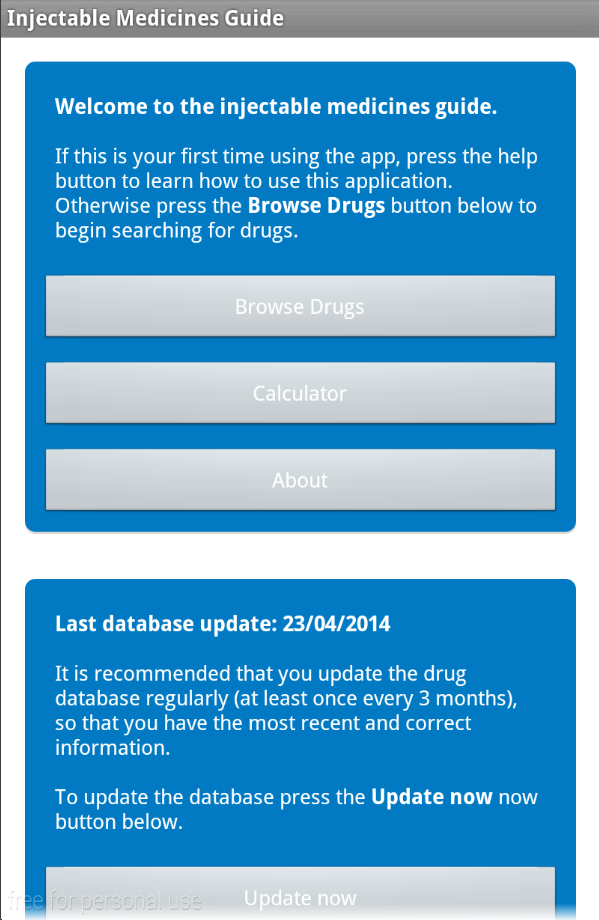
\includegraphics[width=11cm]{Images/screenshots/mainFailed.png}
  \captionof{figure}{Main activity on API 10 before improvement.}
\end{figure}

\section{Completed application screenshots}
This section includes screenshots of the final application, running on two devices, one running API version 10 and another running API version 18.  Android’s style changed greatly between these two versions, the screenshots prove that the application is aesthetically pleasing on both devices.

\begin{figure}[H]
\centering
\begin{minipage}{.5\textwidth}
  \centering
  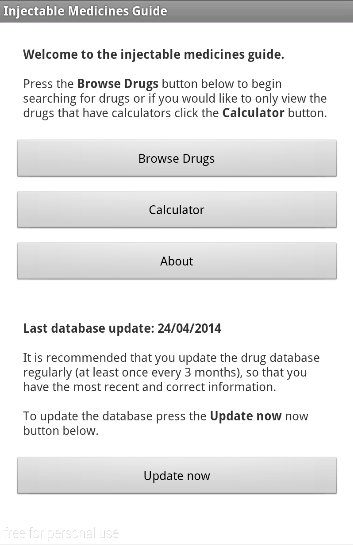
\includegraphics[width=.8\linewidth]{Images/screenshots/API10/main.png}
  \captionof{figure}{Main activity on API 10}
\end{minipage}%
\begin{minipage}{.5\textwidth}
  \centering
  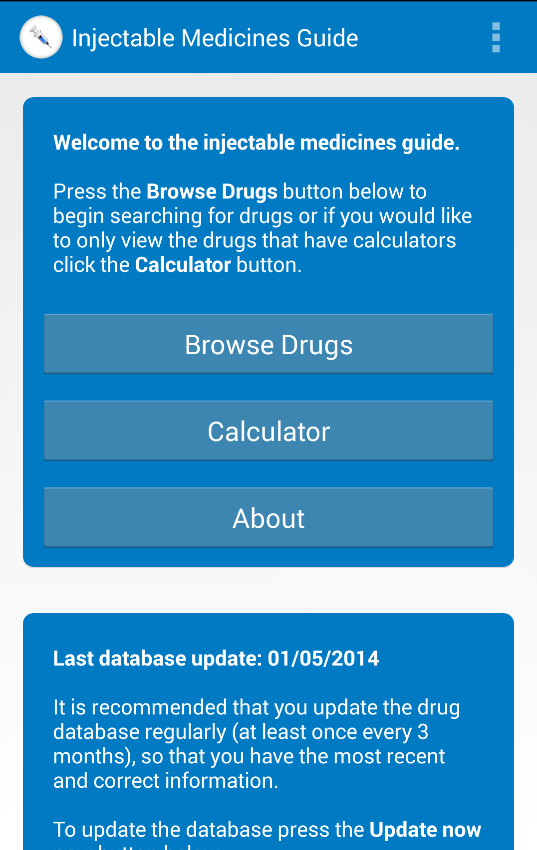
\includegraphics[width=.8\linewidth]{Images/screenshots/API18/main.png}
  \captionof{figure}{Main activity on API 18}
\end{minipage}
\end{figure}

\begin{figure}[H]
\centering
\begin{minipage}{.5\textwidth}
  \centering
  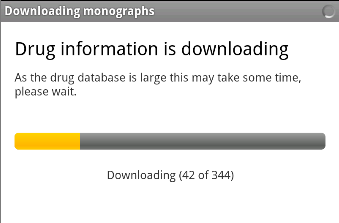
\includegraphics[width=.8\linewidth]{Images/screenshots/API10/download.png}
  \captionof{figure}{Download activity on API 10}
\end{minipage}%
\begin{minipage}{.5\textwidth}
  \centering
  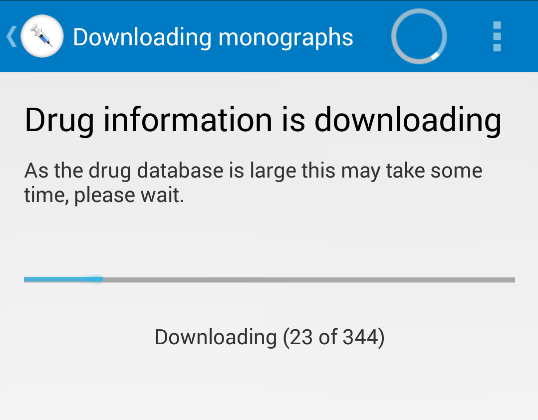
\includegraphics[width=.8\linewidth]{Images/screenshots/API18/download.png}
  \captionof{figure}{Download activity on API 18}
\end{minipage}
\end{figure}

\begin{figure}[H]
\centering
\begin{minipage}{.5\textwidth}
  \centering
  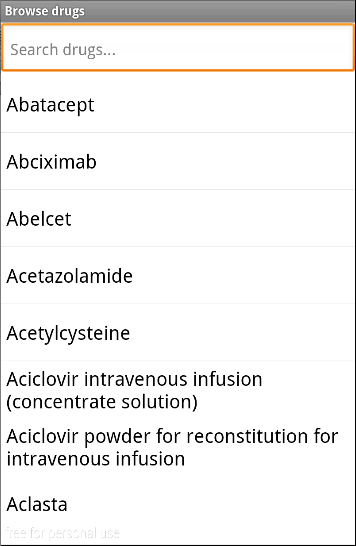
\includegraphics[width=.8\linewidth]{Images/screenshots/API10/browse.png}
  \captionof{figure}{Browse activity on API 10}
\end{minipage}%
\begin{minipage}{.5\textwidth}
  \centering
  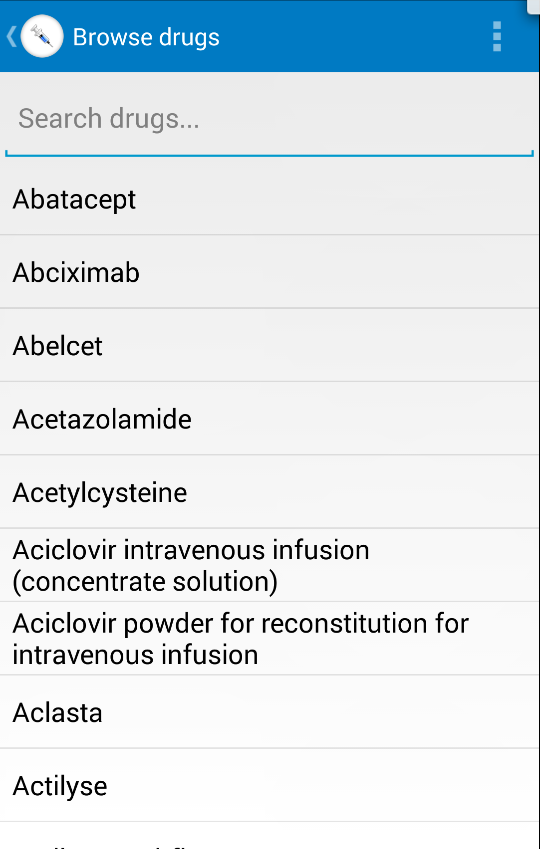
\includegraphics[width=.8\linewidth]{Images/screenshots/API18/browse.png}
  \captionof{figure}{Browse activity on API 18}
\end{minipage}
\end{figure}

\begin{figure}[H]
\centering
\begin{minipage}{.5\textwidth}
  \centering
  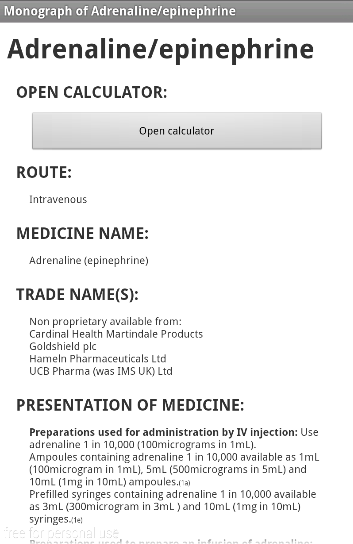
\includegraphics[width=.8\linewidth]{Images/screenshots/API10/view.png}
  \captionof{figure}{View activity on API 10}
\end{minipage}%
\begin{minipage}{.5\textwidth}
  \centering
  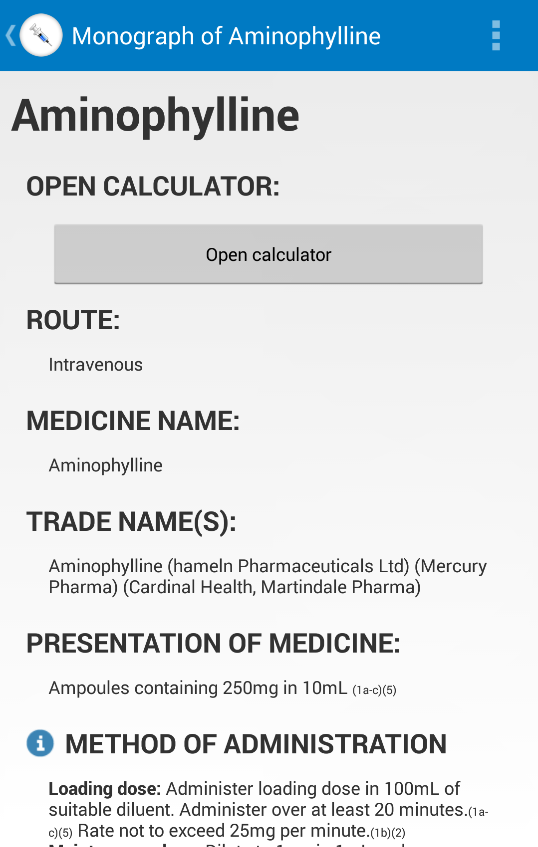
\includegraphics[width=.8\linewidth]{Images/screenshots/API18/view.png}
  \captionof{figure}{View drug activity on API 18}
\end{minipage}
\end{figure}

\begin{figure}[H]
\centering
\begin{minipage}{.5\textwidth}
  \centering
  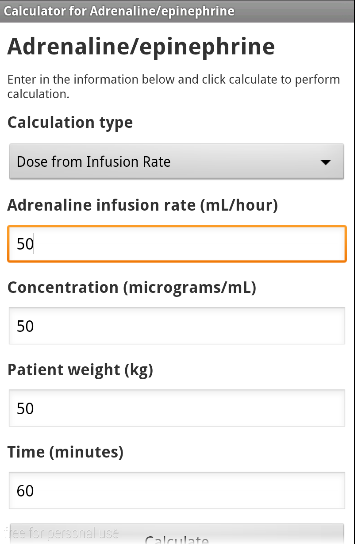
\includegraphics[width=.8\linewidth]{Images/screenshots/API10/calc.png}
  \captionof{figure}{Calculator activity on API 10}
\end{minipage}%
\begin{minipage}{.5\textwidth}
  \centering
  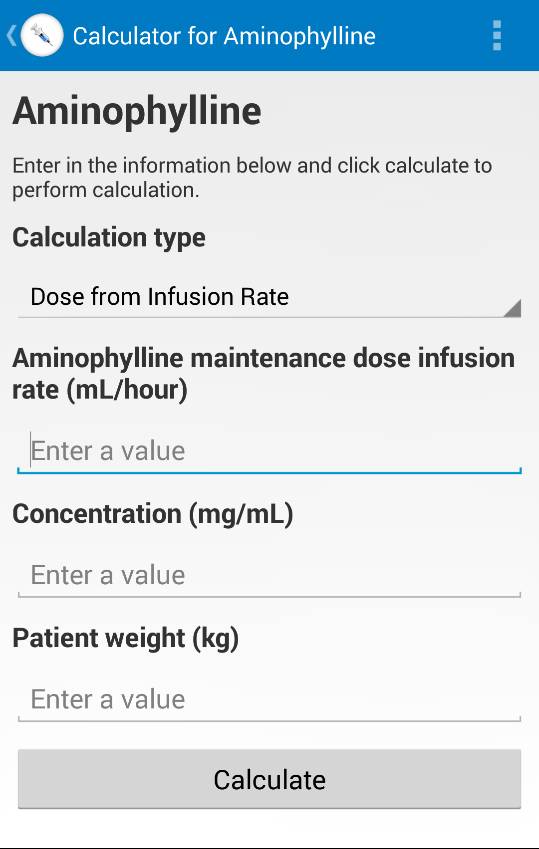
\includegraphics[width=.8\linewidth]{Images/screenshots/API18/calc.png}
  \captionof{figure}{Calculator activity on API 18}
\end{minipage}
\end{figure}

\begin{figure}[H]
\centering
\begin{minipage}{.5\textwidth}
  \centering
  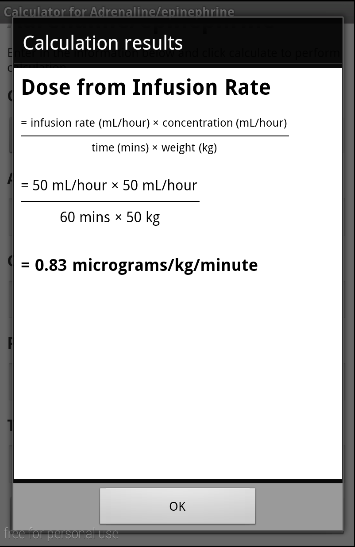
\includegraphics[width=.8\linewidth]{Images/screenshots/API10/calcResult.png}
  \captionof{figure}{Calculator result on API 10}
\end{minipage}%
\begin{minipage}{.5\textwidth}
  \centering
  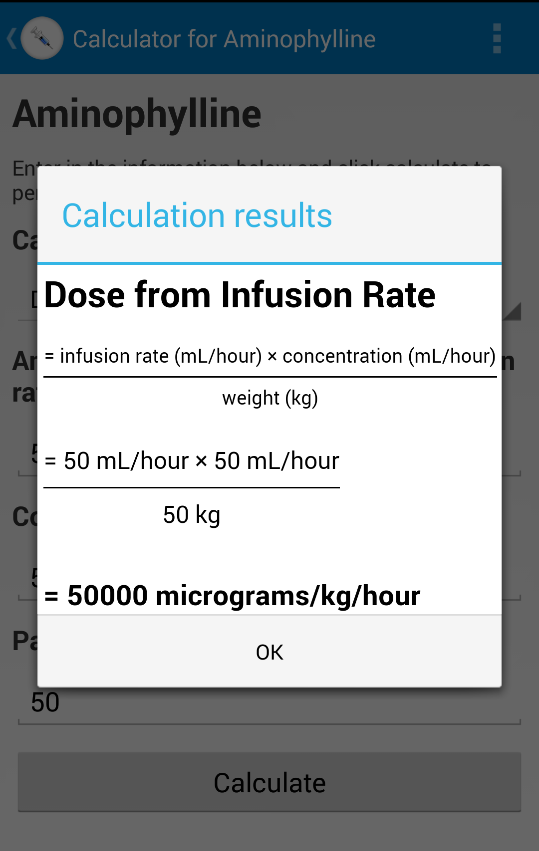
\includegraphics[width=.8\linewidth]{Images/screenshots/API18/calcResult.png}
  \captionof{figure}{Calculator result on API 18}
\end{minipage}
\end{figure}

\chapter{Testing}
Testing is extremely important to the success of any software development project \cite{tdd}. A thorough testing strategy increases robustness and customer confidence within an application. As the application is used to deliver information that will be used by medical staff, it is vital that the application is well tested, as the consequences of poor testing could be fatal. Testing is one of the fundamental steps within the water model \cite{waterfall} and therefore by choosing this methodology testing was enforced. To provide details of the testing carried out during this project a test specification document was produced. This chapter will discus the approach to testing used throughout the project and also describe test strategies used in detail.

\section{Approach to testing}

Testing was used throughout the implementation process to help create a robust and effective application. Originally it was planned to use a test-driven development \cite{tdd} throughout the entire implementation process, but this was later found to be detrimental to the progress of the application.  Although test-driven development was not used throughout the implementation process it was used when developing classes that could potentially be fatal, such as the calculation classes. 

Throughout development the application was ran on a real device and any new features were thoroughly tested, using a variety of behaviours and carefully monitoring the applications state for any anomalies. This approach to implementation allowed for a well-tested application, before any test strategy had been complete.

After the implementation phase of the project had been complete, thorough testing of the application was executed. Unit tests \cite{junit} were written for all classes that had not already had unit tests created. User interface tests were created and executed using android activity unit tests \cite{activity_test}. The application was also stress tested by using Android's exerciser's monkey application \cite{exciser}.

Once the tests had been written, several devices of varying setups were created using the Genymotion emulator \cite{genymotion}. The full list of tests were then executed on each individual device. This ensured that the application runs well on an array of devices.


\section{Test database}

When the testing process began an extra parameter was added to the database constructor, this parameter would allow the application to open a separate database that was identical to the actual database, this separate database could then be used during tests. Having a separate database whilst testing meant that the data could be manipulated without effecting the main application. This was needed, as downloading a new set of data after each test would take a long amount of time.

\section{Unit testing}

The Android SDK \cite{android_sdk} provides classes for unit testing your application. These classes are based off the JUnit framework \cite{junit}, they add extra features such as the ability to access the applications context allowing you to test the database of the application.

Unit tests \cite{junit} were written for every class of the application, testing each public and protected method. Most tests contained multiple assertions, testing that the expected output was returned when correct information is entered and that an error is raised when the incorrect data is entered.

As the unit tests have now been written for all classes, should a developer in the future make any changes to the application, they can execute the unit tests to ensure they have not broken anything. As the unit tests will be provided to the NHS with the source code, they will be able to execute the unit tests for themselves, allowing theming to verify thorough testing was carried out, thus increasing their confidence within the application.

As Android runs on a large amount of devices \cite{phone_market}, unit tests are useful for quickly testing that the application runs as expect across the Android platform. 


\section{Bug that was found due to unit testing}

Test data had been gathered for testing the calculator class. This data was then implemented into unit tests. To ensure the class was well tested a wide spectrum of values were used, including both small and large values.

Within the original implementation of the calculator class I had used floats to store all values and results of the calculation. After executing the unit tests, most tests were succeeding, but few were returning values slightly off the expected value. As the dosage given to patients must be correct to good level accuracy I began investigating the cause of the problem. 

It was found that the issue lay with the data types used, the NHS's website \cite{medusa} used doubles whereas I had used floats. Due to doubles being more accurate than floats, the data types were changed to doubles. The unit test were then executed again and all tests succeeded. 


\section{Automated user interface testing}

Android's activity tests allow you to comprehensively test the user interface of the application \cite{activity_test}. Activity tests simulate the launching of the application's activity \cite{activity_test} and perform a set of unit tests on that activity. These activity unit tests can test a variety of user interface values.

Activity tests were created for every activity. Within the tests each element is checked to ensure that the element is displayed on the screen, the width and height of the element as set correctly, and if the element contains text that the text is set correctly.

Activity tests can test whether an element is visible to the user at that current moment, for example an element may not be visible when the element is displayed at the bottom of a scrollable view. On both the browse drugs and browse calculator activities the search box must be visible to the user at all times. Activity tests were created to ensure the search box is visible to the user.

When the user changes the calculation type on the calculator activity, the dosage and infusion rate fields are toggled, depending on the selected option. As well as this, when a drug calculator is opened for a drug that does not require time or patient weight, the appropriate fields must also be hidden. Activity tests \cite{activity_test} were created to test the calculator activity under a variety of situations to ensure that only the correct fields were displayed.

It was very important to run the activity tests on a variety of devices, this ensured that the user interface functions the same on all devices, without having to manual test each device's user interface.


\section{Automated integration testing}

Due to Android security policies you cannot test the functionality of a user interface element by using activity tests \cite{activity_test}, for example when running an activity test you cannot simulate the user entering text into a text field. Robotium is an automated black-box testing framework \cite{robotium} for Android licenced under the Apache 2 licence \cite{apache_licence}. Robotium allows a developer to implemented black-box integration tests using code \cite{robotium}. There is also a commercially available version of Robotium, which will record user interface actions and monitor the results \cite{robotium}, then automatically generate the Robotium code.

Although automated black-box testing using Robotium would be useful for the project, it was decided that automated tests would not be needed for a project this size. The amount of time spent learning Robotinium and then implementing it, would've taken longer than manual executing the integration tests. If the amount of activities and the functionality within them increase, Robotinium tests should be implemented.


\section{Integration testing}

As Robotinium was not used, a method of testing that the combined units of the application work as expected was needed. To test that the application works as expected a list of integration tests were made and then ran on two devices, one device running API version 19 and the other running API version 8 \cite{froyo}. Using two devices, with varying ages increases the accuracy of the results. To further increase the accuracy of the results the tests would be executed on more devices.

A full list of the integration tests made can be found in the integration testing section of the test results appendix.

\section{Automated stress testing}

Exerciser Monkey \cite{exciser} is a tool provided with the Android SDK \cite{android_sdk}, which is used for stress testing Android applications. The tool simulates a set amount of random events on the device, such as button presses, screen presses, volume changes and screen rotations. The tests are used to ensure that applications run well under stressful tasks and that parts of the application do not throw errors.

It was planned that the application would be installed on a device, then using Exerciser Monkey, execute 5000 random events to the device. The events were executed and the application never crashed, but whilst watching the device I noticed that the exerciser monkey randomly clicked the logout button, from then on the only activity that was tested was the login activity, as it was impossible for the random events to enter a correct username and password. 

It was important for all areas of the application to be tested using this stress tester. Therefore the logout functionality of the application was disabled, which was easy due to modular structure of the application. The Exerciser Monkey was then executed again, simulating 5000s events. The application handled the stress tests well and no errors or timeout warnings were displayed within the console.


\section{Acceptance testing}

To test that the application was at an acceptable level, acceptance testing was carried out. Before sending the application to the NHS for their approval it was vital to test that the application met all of the original functional requirements. This ensured that the application created achieves all of the original goals.

\begin{center}
\begin{longtable}{| l | p{11cm} | c |}
\caption{Table of acceptance testing the functional requirements}\tabularnewline
\hline
   &	\textbf{Functional requirement} & \textbf{PASS/FAIL}   \\ \hline
\textbf{FR 1}                   & \textbf{Authentication}                                                                                                                                                    &           \\ \hline
\textbf{FR 1.1}                 & User must be able to authenticate themselves using their credentials                                                                                                       & PASS      \\ \hline
\textbf{FR 1.2}                 & User must be notified if the password they enter is incorrect                                                                                                              & PASS      \\ \hline
\textbf{FR 1.3}                 & User will be notified if the authentication failed due to connection issues                                                                                                & PASS      \\ \hline
\textbf{FR 1.4}                 & User must be able to logout of the system, removing all data                                                                                                               & PASS      \\ \hline
\textbf{}                       &                                                                                                                                                                            &           \\ \hline
\textbf{FR 2}                   & \textbf{Database synchronisation}                                                                                                                                          &           \\ \hline
\textbf{FR 2.1}                 & After login or when the user presses update the application must truncate all database tables and begin downloading new data                                               & PASS      \\ \hline
\textbf{FR 2.2}                 & Download complete list of drug indexes from database                                                                                                                       & PASS      \\ \hline
\textbf{FR 2.3}                 & Download complete list of drugs and drug information's                                                                                                                     & PASS      \\ \hline
\textbf{FR 2.3}                 & Download all information needed for calculating doses and infusion rates.                                                                                                  & PASS      \\ \hline
\textbf{FR 2.4}                 & Download must still run when the application is in the background                                                                                                          & PASS      \\ \hline
\textbf{}                       &                                                                                                                                                                            &           \\ \hline
\textbf{FR 3}                   & \textbf{Menu options}                                                                                                                                                      &           \\ \hline
\textbf{FR 3.1}                 & Upon pressing the Menu button on the device the user will be presented with a list of available options, which execute tasks (Logout, exit, search…)                       & PASS      \\ \hline
\textbf{}                       &                                                                                                                                                                            &           \\ \hline
\textbf{FR 4}                   & \textbf{Main screen}                                                                                                                                                       &           \\ \hline
\textbf{FR 4.1}                 & Upon successful data download the user will be displayed with a screen where they can navigate to other parts of the application                                           & PASS      \\ \hline
\textbf{FR 4.2}                 & User will be see when an update was last performed, and perform an update from this screen.                                                                                & PASS      \\ \hline
\textbf{}                       &                                                                                                                                                                            &           \\ \hline
\textbf{FR 5}                   & \textbf{Browse drugs}                                                                                                                                                      &           \\ \hline
\textbf{FR 5.1}                 & This screen will allow the user to view a list of all drugs                                                                                                                & PASS      \\ \hline
\textbf{FR 5.2}                 & There will be an input box on this screen, when the user enters text into the input box the results in the list will be filtered to only show results related to the input & PASS      \\ \hline
\textbf{FR 5.3}                 & The user will be able to click a drug in the list to open a new screen displaying the needed information                                                                   & PASS      \\ \hline
\textbf{}                       &                                                                                                                                                                            &           \\ \hline
\textbf{FR 6}                   & \textbf{View drug}                                                                                                                                                         &           \\ \hline
\textbf{FR 6.1}                 & When a drug has been selected the drug and all it's information will be displayed in an easy to read format                                                                & PASS      \\ \hline
\textbf{FR 6.2}                 & Where drug information headers contain help information, a help icon will be displayed next to the header.                                                                 & PASS      \\ \hline
\textbf{FR 6.3}                 & When heading help icon is clicked the helping information will be displayed                                                                                                & PASS      \\ \hline
\textbf{FR 6.4}                 & If the drug had calculator information, then a button to open the calculator should be shown                                                                               & PASS      \\ \hline
\textbf{}                       &                                                                                                                                                                            &           \\ \hline
\textbf{FR 7}                   & \textbf{Browse drugs with calculators}                                                                                                                                     &           \\ \hline
\textbf{FR 7.1}                 & A view similar to the browse drugs view will allow the browsing of drugs that contain calculator information.                                                              & PASS      \\ \hline
\textbf{}                       &                                                                                                                                                                            &           \\ \hline
\textbf{FR 8}                   & \textbf{Calculate dose and infusion rate}                                                                                                                                  &           \\ \hline
\textbf{FR 8.1}                 & The user will be able to select calculation type                                                                                                                           & PASS      \\ \hline
\textbf{FR 8.2}                 & User will be able to enter information required for the calculation                                                                                                        &    PASS       \\ \hline
\textbf{FR 8.3}                 & When the calculate button has been clicked the input will be thoroughly validated                                                                                          & PASS      \\ \hline
\textbf{FR 8.4}                 & After validation the result of the calculation will be displayed to the user                                                                                               & PASS      \\ \hline
\textbf{FR 8.5}                 & The equation and values used to calculate the answer will be neatly displayed to the user                                                                                  & PASS      \\ \hline
\textbf{}                       &                                                                                                                                                                            &           \\ \hline
\textbf{FR 9}                   & \textbf{XML customisability – for developers}                                                                                                                              &           \\ \hline
\textbf{FR 9.1}                 & All text within the application must be changeable through XML files.                                                                                                      & PASS      \\ \hline
\textbf{FR 9.2}                 & The structure of the XML API's provided must be outline within XML files, allowing easy customisation for different API's                                                  & PASS      \\ \hline
\end{longtable}
\end{center}

As shown in the table above the application fulfilled the complete list of functional requirements. The next logical step was to send the compiled APK to the NHS representative for approval.

The representative was very pleased with the final application and only suggested one change, which was to order the calculator's in alphabetical order. This change was implemented and an updated sent to the NHS. Once the changes had been made, the NHS representative demonstrated the application to the IMG Executives Group that consisted of pharmacists and nurse experts, whom stated that the application was intuitive to use and easy to navigate.
 
\section{Acceptance testing feedback}

This section contains the feedback provided by the NHS representative.
\\
\\
\begin{itshape}
"For the first time this year, NHS Wales Informatics Service became involved with Aberystwyth University when we proposed the development of a mobile phone app for the NHS Injectable Medicines Guide (IMG) as a possible dissertation project. The IMG is a website that that provides information on how to prepare and administer injectable drugs and is used by over 90\% of NHS Trusts across the UK by nurses, doctors and pharmacists. It is a major contribution to patient safety and is recommended by the National Patient Safety Agency. We have been under pressure to develop a mobile phone app version of the website.

We supplied an outline design of the app. Aidan was one of two students to select this proposal to take forward as his dissertation. I am providing this feedback as a result of working with Aidan while he has written the software.

My contact with Aidan has been via email and he has always responded promptly to my questions and provided full and accurate answers. Aidan has had to ask us to provide access to the various data sources and I suspect the access that we have provided has not been what he would have chosen but he has always been willing to adapt to what we have provided and work with the our timescales. He has only requested minimal information so he must have worked within his own initiative to complete his work.

And then he delivered the app for us to look at. I was impressed that he had considered how we would implement the software and provided a simple means for us to load the app. Initially we had problems loading the software but Aidan researched the problem and worked with us to resolve the issue which was largely due to the age of our equipment. Implementation and support is a different skill set to development and I was impressed by his problem-solving skills and his persistence in resolving the issue. 

I was bowled over by the app that he has produced; it is well beyond our outline design. He has clearly had to adapt what was essentially an iPhone design to the Android platform and he has produced a design that is very clean and easy to use. He has clearly understood the user interface design principles and I much prefer his design of the pages and the navigation from one function to another over our design.

One aspect of the app is the ability to download and update the data from the central website and to manage the security of this function. Aidan has demonstrated that he understands the security issue and has devised an update that is simple to use but downloads the complex data sets that are involved and has been able to transform the datasets into the information as it appears on the screen, matching across the keys to the each file.

I have demonstrated the app to the IMG Executive Group which consists of Pharmacists from Imperial NHS Trust and an RCN nurse expert on injectable drugs and they were very impressed and found the app intuitive and easy to use. The view was that nurses, for whom very few apps exist and so are not expert users, would find welcome this app and find it easy to navigate.

Overall we are very impressed with the way that Aidan has interacted with us and with the product that he has produced. I am sure he will have an excellent career in software if this is the path that he chooses."
\end{itshape}

\textbf{Robin Burfield, Development Manager, NHS Wales Informatics Service.}

This feedback proves that the application completes its original purpose and that the user interface is clean and easy to use.


\chapter{Evaluation}

This chapter will evaluate the completed project, discuss anything that would have been done differently and outline any future improvements that could be made. 

\section{Evaluation against original goals}

The original goals of the application stated that a native Android application would be created to aid NHS staff in administering injectable medicines to patients. This goal has been achieved as a excellently-working native Android application has been created that, that has been approved by a representative of the NHS to be useful. 

The next goal stated was that the application would be created using the standard user interface library, which is provided with the Android SDK \cite{android_sdk}. Whilst implementing the user interface, no external libraries were used and only standard Android elements were used. This has enabled the final application to work on a large array of Android devices and to be instinctive for a user familiar with Android to use.

As users that may not be technically minded will use this application, the application therefore had to be easy to use. To achieve this the user interface was designed to be clean, simple and self-explanatory for basic users. Using the standard Android user interface library reinforced this goal \cite{android_design}. The feedback left by the NHS confirmed that the final application is both intuitive and easy to use.

As the devices running the applications will not have a constant Internet connection, the application had to download a complete set of data to be used for offline use. The final application does complete this goal and the application can be used within airplane mode, without any degradation of functionality. At first I was worried about the size of the final application with the complete database, but this only amounts to 5 megabytes of disc space, which is very small in comparison to the space available on modern devices. 

The downloading of data and storing that data to the local database had to be possible whilst in the application is in the background, as the download can take several minutes, especially on a mobile data network, the final application achieves this flawlessly. The user can navigate from the application and a notification is placed inside the notification centre alerting the user that the download is still in progress. If an error occurs whilst the application is in the background, when the user re-enters the application they will be asked what action they would like to perform next. 

As NHS staff will be using the application to administer potentially lethal drugs, I wanted to ensure that the application worked as expected. Therefore I planned to thoroughly and vigorously test the application. Throughout the lifecycle of this project testing has been important. I believe the final application has been well tested and should work excellently on a multitude of devices.

The final original goal for the application was to only use publicly accessible libraries, this has been achieved and only two external resources have been used, both of which have been licences under the Apache software licence \cite{apache_licence}.

Overall I believe the application has completed all of the original goals to an excellent standard. I am very pleased with final application and believe I have created a robust, efficient and well-designed piece of software. 


\section{Evaluation against functional requirements}

The requirements set out within the requirements specification were compiled with input from the NHS. Therefore for the application to be deemed successful it was vital that final application implemented the majority of the functional requirements. As shown in the acceptance testing section of the testing chapter, the final application satisfies all of the functional requirements set out in the requirements specification. I believe the finally implemented application has gone above the expectations set out by the original functional requirements.

I am pleased with the list of requirements first set out within the background and analysis stage of the project, they have not had to be modified at any stage in the project. I believe this to be due to thorough project analysis before the project begun.


\section{Time management}

As mentioned in the background chapter, a Gantt chart was created at the start of the project and followed throughout. I did take some time to begin the project due to other freelance work, but by the mid-project demonstration I had caught up with what had been planned. Afterwards the project continued at a steady pace and the project was finished in good time.

The Gantt chart helped motivate me to complete the application in good time, as I could see the tasks that needed to be complete, and how long I had left for each.

\section{Design decisions}

The implemented application follows the design created within the design specification very well. The design utilises the principles brought to the Java language \cite{java} through object orientation and follows many of the software engineering best practices, such as using getters and setters instead of global variables. By using a modulated structure, modules created within this project can be extracted and used within another project with minimal modification. This will be useful if the NHS plan to create multiple applications.

The final implementation only varies slightly from the original design. This was due to deciding to use Robospice services \cite{robospice} over AsyncTasks \cite{async_task}. Due to this, instead of using one class for downloading the complete set of data, multiple classes were built to download and parse individual parts of the dataset. Using Robospice services added many benefits to the final application, such as allowing tasks to be executed in the background and to allow simultaneous downloads through multi-threading. They also improved the design of the application, as separating the downloading and parsing class into separate classes helped to separate classes, which avoided the implementation having a god object anti-pattern.


\section{Methodology}

The methodology used was adapted twice throughout the project. Originally a pure eXtreme programming \cite{xp} was planned, and then the methodology was changed to the waterfall model \cite{waterfall} with test-driven development \cite{tdd} throughout and then later changed to be the waterfall model with test-driven development for critical parts of the system.

Reflecting on the project using the standard waterfall \cite{waterfall} method throughout would’ve been more effective for this project. I wanted to gain experience in using agile methodologies, but using a methodology that I had little experience in, was a hindrance to the project, as extra time was added.

The test driven development \cite{tdd} that I executed did help in finding problems with the calculator class early on, but the problems would’ve still been found during the testing phase, at the end of the waterfall model.


\section{Implementation}

The implemented system is a well-engineered piece of software, which follows software engineering best practices well. The code is split into modules of similar classes and classes have been designed to be as simple as possible, meaning the code is well structured. 

The stress tests shown within the testing chapter show that the application is robust and efficient, as no errors including time out errors were thrown whilst testing under a very large load.

The code style set out within the Android code style guidelines \cite{code_style} has been used throughout the implementation. I have made one modification to this code style; I decided to prefix all private class variables with an underscore. This helped signify whether a variable is local to the method or local to the class.

The code is documented using JavaDoc \cite{javadoc} style comments, which has been compiled into a HTML document, allowing future developers to gain knowledge of the system easily \cite{javadoc}. 

The implementation allows a large amount of the applications to be modified by editing only XML files \cite{xml}. This means the NHS can easily customise the application, even if they do not have any native Android developers.

From the onset of the project I knew that I would not be the sole person to maintain this project and therefore planned to make the project easily maintainable. By using common software engineering principles, using a standard code style and providing extensive comments I believe I this has been achieved.


\section{Changes to the implementation that could be made}

Although the implemented application works as expected there is ways the implementation could be improved. These improvements mainly lie within the classes responsible for downloading the database.

When the application begins downloading the application first downloads the drug indexes, then the drug calculator information and then finally the drug informations are downloaded using multiple threads. When implementing the system, I believed this to be the best method of organising the download. If the application fails to download the drug indexes or the calculator information the applications has to wait for the user to decided what action they would like to perform. Another issue with this approach is that the indexes and calculation are downloaded sequentially and therefore Android’s multithreading capabilities are not used, meaning the process may take longer.

To improve the download task, all services should be pushed to the Robospice service manager when the download activity starts. This will allow the all downloads to start simultaneously and using multiple threads. As the download progress (Download x drugs of y) requires the drug index to be download, a higher priority should be set of the index service and before the download has been finished a standardised message could be used, such as “Download X drugs.”

Another improvement would be to execute the drug letter SQL queries using transactions \cite{sqlite}. Currently drugs are added to the database as soon as they are downloaded. If the download fails whilst mid-way through a letter and the user retries the download, for the drugs that have already been downloaded, the application will attempt to add them again. The drugs are not added to the database, due to primary key constraints on the database, but I believe it is better practice to not have to rely on these constraints. Using a transaction to add drugs starting with each letter will prevent this, as if the download fails the transaction will be cancelled removing all changes.

Currently the user credentials are stored on the device unencrypted, inside the devices user preferences \cite{shared_pref} for the application. This method of storing the credentials is secure under normal operation, but should a malicious user have root access to the device they will be able to extract this data from the user preferences. To secure this, the data needs to be encrypted before being stored on the device.

The key used for the encryption cannot be stored on the device, as that makes the encryption useless, as the hacker will be able to access the key and then be able to decrypt the password. 

There are two methods of securing the key that I considered. One method is to store the key on a server, and then retrieve the key when the key is needed. Another method is to generate the key from a user entered value, such as a PIN, the user can then be asked to enter the PIN whenever the password needs to be decrypted.


\section{Future improvements for the application}

If extra time were available for this project, I would have added extra features and functionality. This section will outline any future improvements that could be added to the system.

\subsection{Cross platform support}

If extra time were provided, making native applications for the other top mobile operating systems would greatly improve the possible reach of the application. Although the models and classes have been written in Java, the design of the classes can be used to implement other operating systems. 

\subsection{Allow the user to add extra notes to drugs}

Although not specifically stated by the NHS, I believe the staff would find the application more useful if they could add notes to an individual drug, these notes would be stored local to the device and would be shown alongside the current drug information. Due to the current database structure this could be implemented easily.

\subsection{Allow the user to add calculator information}

Currently the dataset downloaded for calculations from the NHS only contains around 20 drug calculator informations. Given extra time I would have allowed users to manually enter drug calculator information, thus allowing them to extend their local database. 

This idea could be extended further, and the user could be able to submit there information to the live server, so the information is shared with all users. Due to the nature of the calculations, they would need to be verified by an admin before approval.

\subsection{Partial database update}

To update the database on the current system, the application first deletes all data within the database and then downloads the new data. This was the only method of implementing the update, due to the limitations of the provided API. Given more time I could’ve worked with the NHS to improve the API to allow for partial updates to the database, which would greatly improve the speed of an update.

\subsection{Push notifications of database updates}

Once partial updates had been implemented, it would be beneficial to the user, to get notified via push notifications when an update to the database is available.  This would ensure that the users database is always up to date and would increase user engagement with the application.

\subsection{Ability to reset credentials}

Currently there is no method of resetting the users credentials, should they forget them. Provided extra time, I could have worked with the NHS to create API’s for resetting the users credentials with the application.


\subsection{Allow for online mode}

Some users may not want to download the entire database before using the application. It would be nice to allow user to use the live database from the application, meaning a local copy of the database would not be stored and only informations that is needs is downloaded. Obviously this solution would not work when the user does not have Internet access, but could be useful in places where Internet is available, for example a doctor’s surgery.

% add any additional chapters here

\setemptyheader
\addcontentsline{toc}{chapter}{Appendices}
\chapter*{Appendices}
\pagebreak

% start the appendix - sets up different numbering
\fancypagestyle{plain}{%
%\fancyhf{} % clear all header and footer fields
\fancyhead[L]{\textsl{Appendix\ \thechapter}}
\fancyhead[R]{\textsl{\leftmark}}}

\appendix
\fancyhead[L]{\textsl{Appendix\ \thechapter}}
\fancyhead[R]{\textsl{\leftmark}}
\fancyhead[C]{}
\fancyfoot[C]{\thepage}
\renewcommand{\headrulewidth}{0.4pt}
\renewcommand{\chaptermark}[1]{\markboth{#1}{}}

\fancyhead[L]{\textsl{Appendix\ \thechapter}}
\fancyhead[R]{\textsl{\leftmark}}
\fancyfoot[C]{{\thepage} of \pageref{LastPage}}

% include any appendices here
\chapter{Third-Party Code and Libraries}
\begin{description}
\item[Android SDK Library]
The Android SDK Library \cite{android_sdk} has been to create a native Android application. This library has provided the application with many useful functions, such as the user interface and database interactons. This 

\item[Robospice Library]
The Robospice Library \cite{robospice} was used to create asynchronous download services. These services allowed the data download task to run in the background. Robospice is licenced under the Apache 2.0 licence \cite{apache_licence}. This library was used without modification, although one class was duplicated and used within my project to add extra functionalilty.

\item[Junit]
The JUnit framework \cite{junit} was used to execute unit tests on the completed implementation.
\end{description}
\chapter{Code samples}

\section{Random Number Generator}

The Bayes Durham Shuffle ensures that the psuedo random numbers used in the simulation are further shuffled, ensuring minimal correlation between subsequent random outputs \cite{NumericalRecipes}.

\begin{verbatim}
 #define IM1 2147483563
 #define IM2 2147483399
 #define AM (1.0/IM1)
 #define IMM1 (IM1-1)
 #define IA1 40014
 #define IA2 40692 
 #define IQ1 53668
 #define IQ2 52774
 #define IR1 12211
 #define IR2 3791
 #define NTAB 32
 #define NDIV (1+IMM1/NTAB)
 #define EPS 1.2e-7
 #define RNMX (1.0 - EPS)
 
 double ran2(long *idum)
 {
   /*---------------------------------------------------*/
   /* Minimum Standard Random Number Generator          */
   /* Taken from Numerical recipies in C                */
   /* Based on Park and Miller with Bays Durham Shuffle */
   /* Coupled Schrage methods for extra periodicity     */
   /* Always call with negative number to initialise    */
   /*---------------------------------------------------*/	
 
   int j;
   long k;
   static long idum2=123456789;
   static long iy=0;
   static long iv[NTAB];
   double temp;
 
   if (*idum <=0)
   {
     if (-(*idum) < 1)
     {
       *idum = 1;
     }else
     {
       *idum = -(*idum);
     }
     idum2=(*idum);
     for (j=NTAB+7;j>=0;j--)
     {
       k = (*idum)/IQ1;
       *idum = IA1 *(*idum-k*IQ1) - IR1*k;
       if (*idum < 0)
       {
         *idum += IM1;
       }
       if (j < NTAB)
       {
         iv[j] = *idum;
       }
     }
     iy = iv[0];	
   }
   k = (*idum)/IQ1;
   *idum = IA1*(*idum-k*IQ1) - IR1*k;
   if (*idum < 0)
   {
     *idum += IM1;
   }
   k = (idum2)/IQ2;
   idum2 = IA2*(idum2-k*IQ2) - IR2*k;
   if (idum2 < 0)
   {
     idum2 += IM2;
   }
   j = iy/NDIV;
   iy=iv[j] - idum2;
   iv[j] = *idum;
   if (iy < 1)
   {
     iy += IMM1;
   }
   if ((temp=AM*iy) > RNMX)
   {
     return RNMX;
   }else
   {
     return temp;	
   }
 }
 
\end{verbatim}



\setemptyheader
\chapter*{End of appendices}
\pagebreak


\fancypagestyle{plain}{%
   \fancyhead{} %[C]{Annotated Bibliography}
   \fancyfoot[C]{{\thepage} of \pageref{LastPage}} % except the center
   \renewcommand{\headrulewidth}{0pt}
   \renewcommand{\footrulewidth}{0pt}
}

\setemptyheader

\nocite{*} % include everything from the bibliography, irrespective of whether it has been referenced.

% the following line is included so that the bibliography is also shown in the table of contents. There is the possibility that this is added to the previous page for the bibliography. To address this, a newline is added so that it appears on the first page for the bibliography. 
\addcontentsline{toc}{chapter}{Annotated Bibliography} % Adds References to contents page

%
% example of including an annotated bibliography. The current style is an author date one. If you want to change, comment out the line and uncomment the subsequent line. You should also modify the packages included at the top (see the notes earlier in the file) and then trash your aux files and re-run. 
%\bibliographystyle{authordate2annot}
\bibliographystyle{IEEEannot}
\renewcommand{\bibname}{Annotated Bibliography} 
\bibliography{References/references} % References file


\end{document}
